\chapter{Metodologia}\label{cap:metodologia}

\begin{citacao}
O saber só existe como pluralidade de saberes, tal como a ignorância só existe como pluralidade de ignorâncias. As possibilidades e os limites de compreensão e de acção de cada saber só podem ser conhecidas na medida em que cada saber se propuser uma comparação com outros saberes. Essa comparação é sempre uma versão contraída da diversidade epistemológica do mundo, já que esta é infinita. É, pois, uma comparação limitada, mas é também o modo de pressionar ao extremo os limites e, de algum modo, de os ultrapassar ou deslocar. Nessa comparação consiste o que designo por ecologia de saberes. (\ldots) Sendo sempre limitado o conjunto de saberes que integra a ecologia dos saberes há que definir como se consitituem esses conjuntos. \textbf{À partida, é possível um número ilimitado de ecologia de saberes, tão ilimitado quanto o da diversidade epistemológica do mundo. Cada exercício de ecologia de saberes implica uma selecção de saberes e um campo de interacção onde o exercício tem lugar}. \cite[p.~28-30]{santos_filosofia_2008}.
\end{citacao}

\citeonline[p.~11--12]{santos_filosofia_2008} elabora a imagem mental \ver{sec:imagem_mental} de uma feira do conhecimento, onde teorias  são antropomorfizadas, escravizadas e vendidas:\ ``determinismo, livre arbítrio,universalismo, relativismo, realismo, construtivismo, marxismo, liberalismo, neoliberalismo, estruturalismo, pós-estruturalismo, modernismo, pós-modernismo, colonialismo, pós-colonialismo, etc.''. As idéias perderam a utilidade para os ex-adeptos, que não estão mais interessados em comprá-las. E vendem aos que supõe algum valor. Para efetuar a venda, é necessário estabelecer uma relação de custo-benefício, definida por meio das respostas às perguntas: ``qual a utilidade que esta ou aquela teoria poderá ter para mim? Qual o preço?''. A valorização ocorre quando esta teoria se torna mais apelativa que aquela: o preço-teto estabelecido é a verdade da resposta. A livre-associação dos vendedores buscará regulamentar as compras e vendas de conhecimentos conforme seu interesse mais fundamental: se todas teorias forem vendidas não existirá teoria para se vender amanhã.

É possível pensar que esta metáfora de um Mercado contemporâneo do conhecimento é uma ficção científica forçada. Mas Santos esclarece que este tema é anterior à formação do espírito científico moderno: no texto satírico \emph{A venda de filosofias} (165), Luciano de Samósata (125 -- 181?),  escreve sobre um mercado estimulado por Zeus e gerenciado por Hermes. Neste mercado é possível comprar escravos como  ``(\ldots) epicurismo, estoicismo, cepticismo peripatético.'':

\begin{citacao}
Hermes atrai os potenciais compradores, todos comerciantes, gritando alto e bom som “À venda! Uma variedade sortida de filosofias vivas! Posições de todo o tipo! Pagamento à vista ou mediante garantia!” (1905: 190). A “mercadoria” vai sendo exposta, os comerciantes vão chegando e têm o direito de interrogar cada uma das filosofias à venda, começando invariavelmente com a pergunta pela utilidade para o comprador e a sua família ou grupo. O preço é estabelecido por Zeus que, por vezes, se limita a aceitar ofertas feitas pelos comerciantes compradores. A venda tem pleno êxito e Hermes termina, ordenando às teorias que deixem de oferecer resistência e sigam com os seus compradores, ao mesmo tempo que avisa o público: “Senhores, esperamos vê-los amanhã. Estaremos oferecendo novos lotes úteis para homens comuns, artistas e comerciantes”   
\end{citacao}

O texto satírico de Luciano de Samósata, descrito por Santos, antecipa em séculos um Mercado regulamentado do conhecimento, formado por ``universidades, editoras, resenhas, revistas especializadas, congressos, jornais de divulgação cultural, catálogos, \emph{amazon.com},(\ldots)''\cite[p.~12--13]{santos_filosofia_2008}. A universidade é um caso particular, pois é o setor de validação deste conhecimento.  Válido do ponto de vista do que é possível descrever cientificamente. O que queremos dizer com científico, através de uma metáfora farmacêutica: \metafora{O ideal é o remédio monofuncional, o substantivo seguido de um só adjetivo}\footnote{Bachelard, G. \emph{A Formação do Espírito Científico: contribuição para a psicanálise do conhecimento}. p.143, 1938. Grifo em caixa-alta nosso.}. Com isso queremos dizer que a prática de reduzir conceitos cada vez mais, em nossa época, enfraquece qualquer resposta a ser produzida. Para Santos é fraca em comparação aos problemas contemporâneos que podem ser vivenciados em situações de risco. Indolor para aquele que produz o conhecimento, mas dolorida para aquele que está do outro lado da linha do conhecimento.

O \emph{conhecimento ortopédico} que é historicamente produzido por um Norte global é traduzido em política. Estas políticas são o dispositivo de manutenção de poderes exercidos no Sul global, através do Sul Imperial. Para descrever os conceitos e suas metáforas, conhecimento-ortiopédico, Norte e Sul Global/Imperial, colocaremos, nos dois próximos parágrafos, o primeiro termo entre-aspas e o segundo em caixa-alta \cite[p.~32]{McLean2011}. Não é nossa intenção levantar todos problemas epistemplógicos discutidos por \citeonline{santos_abissal_2007,santos_filosofia_2008}. Antes, este capítulo propõe a investigação de um pensamento ortopédico produzido em um Norte global, em relação à improvisação de códigos.

\section{Conceito de Pensamento Ortopédico}

Três conceitos auxiliares ajudam a compreender o termo ``conhecimento ortopédico''. O primeiro se relaciona com a metáfora do \scriptsize MÉDICO ESPECIALISTA EM CORRIGIR OU EVITAR AS DEFORMIDADES DO CORPO \normalsize \disponivelem{http://www.priberam.pt/dlpo/ortopedia}. O segundo é a \emph{a razão indolente}, que ilustra uma \scriptsize ``FRIEZA EMOCIONAL'' QUANTO AO PROCESSO DE CORREÇÃO\normalsize : ``A carência a respeito da finitude transforma-se num problema técnico-científico, enquanto a carência a respeito da diversidade infinita é ignorada como um não-problema.'' \cite[p.~15]{santos_filosofia_2008}. O terceiro é \emph{o pensamento abissal} \cite[p.~1--4]{santos_abissal_2007}, \scriptsize UMA DIFERENÇA DE DISTÂNCIA ESPACIAL ENTRE DOIS PONTOS \normalsize:

\begin{citacao}
Consiste num sistema de distinções visíveis e invisíveis, sendo que as invisíveis fundamentam as visíveis. As distinções invisíveis são estabelecidas através de linhas radicais que dividem a realidade social em dois universos distintos: o universo  'deste lado da linha' e o universo 'do outro lado da linha'. A divisão é tal que 'o outro lado da linha' desaparece enquanto realidade, torna-se inexistente, e é mesmo produzido como inexistente. (\ldots) \textbf{O pensamento abissal moderno salienta-se pela sua capacidade de produzir e radicalizar distinções.} Contudo, por mais radicais que sejam estas distinções e por mais dramáticas que possam ser as consequências de estar de um ou do outro dos lados destas distinções, elas têm em comum o facto de pertencerem a este lado da linha e de se combinarem para tornar invisível a linha abissal na qual estão fundadas. \end{citacao}

A metáfora para os conceitos ``Norte global'' e ``Sul Global'' podem ser classificadas como \emph{conceitos orientados espacialmente}\footnote{\loccit{McLean2011}.}. Isto é, se as imagens mentais de ``Norte'' e ``Sul'' remetem à localização de países representados em um mapa acima da Linha do Equador, é antes uma metáfora para \metafora{um grupo de elites sócio-econômicas não-atentas ao outro lado da linha}.  

\section{Objetivo}

Não é nossa intenção discutir todos os problemas levantados por Santos. A digressão da metáfora \metafora{conhecimento consificado e simbolicamente capitalizado} ilustra, em uma esfera diversa da presente pesquisa, uma prática de bricolagem realizada na improvisação de códigos. Uma dessas bricolagens considera o estudo da Improvisação Musical, sob o ponto de vista das ciências cognitivas e computacionais. O \emph{Universo de Conceitos}, investigado neste capítulo, é um desses pensamentos abissais. De maneira curiosa, contrasta com a proposta de Santos, a \emph{Ecologia de Saberes}, uma metáfora para \metafora{um complexo sistema de comunidades de conhecimentos vivos}.

\section{Justificativa}

 A manutenção deste conhecimento, nesta forma, não é interessante para o Sul global. Desenvolve um pensamento cirúrgico no conceito ``criatividade na improvisação de códigos musicais''. Mas compramos a idéia por que supomos algum valor \cite[p.~20]{santos_filosofia_2008}, ``Afinal, se há compra e venda é porque as teorias e disciplinas têm alguma utilidade. Doutro modo, seriam simplesmente deitadas ao lixo.''. O preço estabelecido não é grande, e só uma parte da teoria será utilizada para a análise de um trecho de uma improvisação musical discutido no \autoref{cap:estudos_de_caso}.

\section{Criatividade}\label{sec:sistemas_criativos}

\begin{citacao}
Por definição, criatividade cria, i.e., produz alguma coisa nova. Mas se estamos comprometidos com uma abordagem mecanicista do mundo -- nenhum milagre é permitido -- iremos acreditar que tudo o que ocorre é, em princípio,  previsível. Iremos acreditar também que qualquer coisa nova deve ser construída de componentes existentes. Isso implica que nada pode ser intrinsicamente novo. \cite[p.~2]{thornton_quantitative_2007}\footnote{Tradução de \emph{By definition, creativity creates, i.e., it produces something new. But if we are committed to a mechanistic account of the world — no miracles allowed — we believe that everything that occurs is predictable in principle. We also believe that any new thing must be constructed from existing components. This implies that nothing can ever be intrinsically new.}}
\end{citacao}
 
``Mas o que exatamente é criatividade?'' \cite[p.~117--127]{McLean2011}. A definição acima começa com uma definição circular. Esta circularidade destaca a continuidade de uma atividade por trás de um trabalho, considerado por mais de uma pessoa, como criativo.  O processo de trabalho realizado por um agente é considerado criativo por outra pessoa quando esta cria novos \emph{espaços conceituais}. Por exemplo, um paradigma de criatividade ilustrado por McLean ilustra a \emph{Prática Reflexiva} de Paul Klee, que perturba o vazio do quadro através do movimento inicial com sua mão, e após observar o que fez, julga (e se julga) dentro de seu próprio sistema estético. A auto-crítica o faz reconsiderar o movimento, ou o faz complementar o movimento. Um novo julgamento é realizado, mas nunca descontinuado \ver{fig:feedback}.

  \begin{figure}[!h]
    \centering
    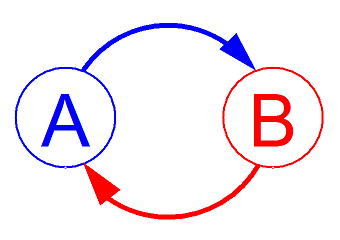
\includegraphics[scale=0.5]{imagens/Simple_Feedback_02.png}
    \caption{Retroalimentação simples entre duas partes. \textbf{Fonte}: wikimedia.org}
    \label{fig:feedback}
  \end{figure}

Mas a tarefa do improvisador-programador é diversa do pintor. Sua tentativa de expressão é realizada na forma de texto escrito em uma forma lógica, e não na forma de tinta a óleo. Este caso será ilustrado musicalmente no \autoref{cap:estudos_de_caso}. A posição defendida por McLean utiliza a representação geométrica de relações entre \emph{conceitos} pré-existentes na pessoa que percebe algo, formando novos \emph{conceitos} e reformulando seu \emph{espaço conceitual}. Por hora, vamos definir o que é uma Imagem Mental e Espaço Conceitual.

\subsection{Imagem Mental e Conceito para improvisador-programador}\label{sec:imagem_mental}

Definir verbalmente, ``imagem mental'', em termos visuais, estabelece uma relação entre a observação e a verbalização. No entanto esta não é a única relação. Para \citeonline[p.~24]{McLean2011}, imagens mentais se relacionam com quaisquer estados quase-perceptuais: \traducao{Por exemplo o uso de entonação prosódica na fala é \emph{paralinguística}, não inteiramente natada em texto escrito, mas ainda assim simboliza um conteúdo significativo.}{For example the use of prosodic intonation in speech is \emph{paralinguistic}, not entirely notated in written text, yet symbolising meaningful content}

A teoria da \emph{Codificação Dual} de Alan Paivio\footnote{\emph{Mental representations: A Dual Coding Approach (Oxford Psychologyu Series). Oxford University Press, USA.}} \cite[p.~25--29]{McLean2011} estabelece uma relação de colaboração corrente entre as hierarquias de códigos de percepção: \traducao{humanos são capazes de compreender linguagem enquanto simultaneamente atendem às imagens. }{humans are able to comprehend language while simultaneously attending to imagery.}:

\begin{citacao}
\traducao{Seu $[$Paivio$]$ argumento não é que existem dois códigos, mas sim que existe uma hierarquia de códigos, que se ramificam no topo em códigos lingüísticos discretos e códigos de percepção contínua, que Paivio nomesia como \emph {logogens} e \emph{imagens} respectivamente.}{His contention is not that there are two codes, but rather that there is a hierarchy of code, which branch at the top into discrete linguistic codes and contionuous perceptual codes, which Paivio names \emph{logogens} and \emph{imagens} respectively}
\end{citacao}

Um sistema visual geométrico auxilia entender outro sistema de símbolos discretos ordenados por regras gramaticais. De um lado, a imagem mental é elaborada de maneira geométrica simultaneamente com o texto falado ou escrito. Para \citeonline[p.~125]{McLean2011} é a fase de \emph{elaboração}, como por exemplo, a leitura deste texto. 

Por outro, o domínio textual do improvisador-programador é diverso de um literato. Na improvisação de códigos, o texto é escrito para formalizar operações, que posteriormente serão compilados para um código compreensível pela máquina. Exemplificamos como um código em branco, cuja experiência se dará com o microfone do \emph{laptop} do leitor. Esta é \emph{estratégia transversal} em atividade \ver{ex:supercollider}

\begin{example}

\metafora{imagem mental}: em uma performance para \emph{laptop}, expressaremos uma microfonia cujo timbre seja auto-modificado. Primeiro criamos um espaço de performance (1); escrevemos um código para o microfone (2); em seguida podemos aplicar uma sequência de atrasos controlados (2)

  \begin{minted}{javascript}
    // (1) 
    s.boot                   // ligar o servidor de audio
    p = ProxySpace.new       // ambiente virtual de performance 
    p.fadeTime = 5           // fadein/fadeout entre cada modificacao

    // (2)
    ~mic={AudioIn.ar([0,1])} // Estereofonico

    // (3)=microfone, tempo de delay maximo, tempo 
    ~d = {CombL.ar(~mic.ar, 1, 0.5, 0.5, 1, ~mic.ar*0.1)}
    
  \end{minted}
\end{example}




\subsection{Espaços conceituais}\label{sec:componentes}

 \citeonline[p.~450]{wiggins_framework_2006} sumarizou e formalizou os \emph{Espaços Conceituais} de \citeonline{boden_creative_1990} segundo tais formalizações geométricas. Segundo o autor, \traducao{Boden concebe o processo de criatividade como uma identificação e/ou localização de novos objetos conceituais em um espaço conceitual.}{Boden conceives the process of creativity as the identification and/or location of new conceptual objects in a conceptual space.}. Uma definição semelhante de \citeonline[p.~2]{thornton_quantitative_2007} reafirma a criação de uma imagem mental de uma \emph{metáfora} (que pode situar sons, palavras, imagens, cheiros,tato,gostos):\traducao{Qualquer ato criativo é fundado na conceitualização ou realização de um ponto dentro de um espaço conceitual particular}{Any creative act is thus founded on conceptualisation or the realisation of a point within a particular ‘conceptual space’}. 

Três processos-chave são considerados: a primeira é a formação de um espaço de conceitos diante de imagem mental que o improvisador-programador experenciou. 

\begin{figure}[!h]
  \centering
  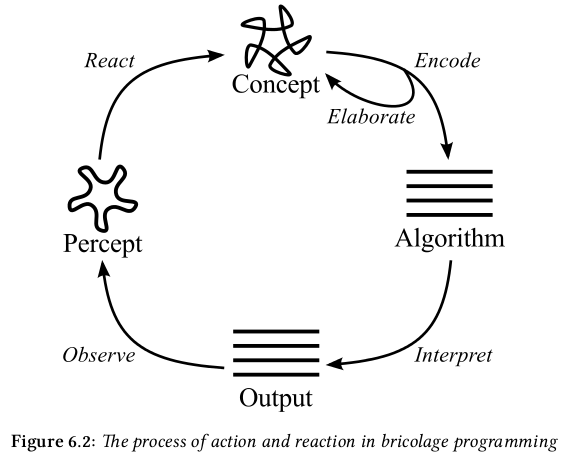
\includegraphics[scale=1]{imagens/processo_criativo.png}
  \caption{Modelo de bricolagem para o processo criativo realizado por um artista-programador. \textbf{Fonte}: \citeonline[p.~122]{McLean2011}. }
  \label{fig:processo_criativo}
\end{figure}

\begin{citacao}
\traducao{A Figura 6.2 $[$\autoref{fig:processo_criativo}$]$ caracteriza a programação por bricolagem como um laço retroalimentado envolvendo o algoritmo escrito, sua interpretação, e a percepção do programador e sua reação do resultado ou comportamento $[$do algoritmo$]$. (\ldots). No começo o programador tem um conceito meio-formado que só atinge consistência interna através do processo de ser expresso como um algoritmo. O laço interno é onde o programador elabora o objetivo de suas imaginações, e o laço externo é onde essa trajetória está fundamentada na pragmática do que elas realmente têm que fazer. Através deste processo ambos algoritmos e conceitos são desenvolvidos até que o programador sinta que um se aplica com o outro, ou de outra forma julga o processo criativo finalizado.
}{
Figure 6.2 characterises bricolage programming as a creative feedback loop encompassing the written algorithm, its interpretation, and the programmer’s perception and reaction to its output or behaviour. (\ldots). At the beginning, the programmer may have a half-formed concept, which only reaches internal consistency through the process of being expressed as an algorithm. The inner loop is where the programmer elaborates upon their imagination of what might be, and the outer where this trajectory is grounded in the pragmatics of what they have actually made. Through this process both algorithm and concept are developed, until the programmer feels they accord with one another, or otherwise judges the creative process to be finished.
}  
\end{citacao}

\subsubsection{Processo criativo como bricolagem}\label{sec:bricolagem}


\subsubsection{Conceito}

We can think of ourselves as spatial beings able to simulate a linguistic environment to conduct abstract thought and open
channels of communication. p.124 McLean2011

\subsubsection{Metáfora}

\section{Sistemas criativos}\label{sec:sistemas}

\begin{table}[!h]
\caption{Definições formais de criatividade por \citeonline[p.~451]{wiggins_framework_2006}}
\small
    \begin{tabular}{ | p{4cm} | p{11.25cm} |}
    \hline 
    \hline 

    \tiny{Criatividade} 
    & \tiny{``A performance de tarefas que, quando executados por um humano, são consideradas criativas''  \tablefootnote{Tradução de \emph{The performance of tasks which, if performed by a human, would be deemed creative.}.}} \\
    \hline

    \tiny{Computação criativa} 
    & \tiny{``O estudo e suporte, através de meios e métodos computacionais, do comportamento exibido por sistemas naturais e artificiais, que são considerados criativos''. \tablefootnote{Tradução de \emph{The study and support, through computational means and methods, of behaviour exhibited by natural and artificial systems, which would be deemed creative if exhibited by humans.}.}} \\
    \hline

    \tiny{Sistemas criativos} 
    & \tiny{``Uma coleção de processos, naturais ou automáticos, que são capazes de alcançarem ou simularem comportamentos que em humanos seria considerado criativo''} \\
    \hline

    \tiny{Comportamento Criativo} 
    & \tiny{``Um ou mais dos comportamentos exibidos por um sistema criativo''\tablefootnote{Tradução de \emph{One or more of the behaviours exhibited by a creative system.}}} \\
    \hline
   
    \end{tabular}
\label{tab:criatividade}
\end{table}

\subsection{Quadro Conceitual de sistemas criativos}\label{sec:csf}

Uma maneira adequada de descrever um sistema criativo (ou parte dele) considera um \emph{Universo de Conceitos}:

\begin{citacao}
O universo, $\mathcal{U}$, é um espaço multidimensional, no qual dimensões são capazes de representar qualquer coisa, e todos os possíveis conceitos distintos correspondentes àqueles pontos em $\mathcal{U}$ (\ldots) Para tornar a proposta um espaço-tipo possível, permitirei que $\mathcal{U}$ contenha todos os conceitos abstratos, bem como os concretos, e que é possível representar os artefatos tanto completos e incompletos \cite[p.~451]{wiggins_framework_2006}.\footnote{Tradução de \emph{The universe, U, is a multidimensional space, whose dimensions are capable of representing anything, and all possible distinct concepts correspond with distinct points in U. (\ldots) To make the proposal as state-spacelike as possible, I allow that U contains all abstract concepts as well as all concrete ones, and that it is therefore possible to represent both complete and incomplete artefacts}}
\end{citacao}

Wiggins esclarece que Boden não reconhece de forma explícita $\mathcal{U}$, ``ela borra a distinção entre as regras que determinam a adesão do espaço (\ldots) e outras disposições que possam permitir a construção e/ou detecção de um conceito representado por um ponto no espaço'' (\emph{Idem, ibdem}).

Espaços conceituais $\mathcal{C}$, finitos ou infinitos são definidos como restrições de um universo $\mathcal{U}$, caracterizando um conjunto não-determinístico de conhecimentos: \traducao{A noção-chave na teoria de Boden é aquele do espaço conceitual. Enquanto nenhuma definição formal é provida, é comum interpretar esta frase literalmente, tomando o espaço conceitual sendo um espaço de conceitualizações, ou representações de conceitos \cite[p~.7]{thornton_quantitative_2007}.}{The key notion in Boden’s theory is that of the conceptual space. While no formal definition has been provided, it is common to interpret the phrase literally, taking the conceptual space to be a space of conceptualisations or concept representations.}

\citeonline{mclean_music_2006} ainda descreve regras que validam concepções diferentes entre espaços conceituais $\mathcal{C}$ diversos em um Universo de Conceitos $\mathcal{U}$ (ver \autoref{tab:universodeconceitos}).

\begin{table}[!h]
\caption{Definições formais do Universo de possibilidades de \citeonline{wiggins_framework_2006}, ou Universo de Conceitos por \citeonline{mclean_music_2006}.}
\small
    \begin{tabular}{ | p{4.25cm} | p{5.25cm} | p{5.25cm} |}
    \hline 
    \hline 

    Representação
    & \tiny{Nome}     
    & \tiny{Significado} \\
    \hline

    $c$
    & \tiny{Conceito} 
    & \tiny{Uma instância de um conceito, abstrato ou concreto \cite{wiggins_framework_2006}}. \\
    \hline

    $\mathcal{U}$
    & \tiny{Universo de Conceitos} 
    & \tiny{Superconjunto não restrito de conceitos. \cite{wiggins_framework_2006}. ``Um universo de todos conceitos possíveis'' \cite{mclean_music_2006} \tablefootnote{Tradução de \emph{A universe of all possible concepts}.}}\\
    \hline

    $\mathcal{L}$
    & \tiny{Linguagem} 
    & \tiny{Linguagem utilizada para expressar regras.} \\
    \hline

    $\mathcal{A}$
    & \tiny{Alfabeto} 
    & \tiny{Alfabeto da linguagen que contêm caracteres apropriadospara expressão das regras} \\
    \hline

    $\mathcal{R}$
    & \tiny{Regras de validação} 
    & \tiny{Validam os conceitos em um universo, se apropriados ou não para o espaço trabalhado.} \\
    \hline

    $[[.]]$
    & \tiny{Função de interpretação} 
    & \tiny{``Uma função parcial de $\mathcal{L}$ para funções que resultam em números reais entre [0, 1] (\ldots) 0.5 $[$ou maior$]$ significa uma verdade booleana e menos que 0.5 siginifica uma falsidade booleana; a necessidade disso para valores reais se tornará clara abaixo'' \cite[p.~452]{wiggins_framework_2006}\tablefootnote{Tradução de \emph{(\ldots) a partial function from $\mathcal{L}$ to functions yielding real numbers in [0, 1]. (\ldots) 0.5 to mean Boolean true and less than 0.5 to mean Boolean false; the need for the real values will become clear below}.}}\\
    \hline

     $[[\mathcal{R}]]$
    & \tiny{Regras de validação} 
    & \tiny{``Uma função que interpreta $\mathcal{R}$, resultando em uma função indicando aderência ao conceito em $\mathcal{R}$''\tablefootnote{Tradução de \emph{A function interpreting $\mathcal{R}$, resulting in a function indicating adherence of a concept to $\mathcal{R}$}}} \\
    \hline

     $\mathcal{C} = [[\mathcal{R}]](\mathcal{U}) $
    & \tiny{Espaço Conceitual} 
    & \tiny{``Todos espaços conceituais são um subconjunto não-estrito de $\mathcal{U}$''\tablefootnote{Tradução de \emph{All conceptual spaces are non-strict subset}.}. Um subconjunto contido em $\mathcal{U}$ \cite{wiggins_framework_2006}. Uma função que interpreta $\mathcal{R}$, resultando em uma função que indica aderência ao conceito em $\mathcal{R}$ \tablefootnote{Tradução de \emph{A function interpreting $\mathcal{R}$, resulting in a function indicating adherence of a concept to $\mathcal{R}$}.} } \\
    \hline

    $\mathcal{T}$
    & \tiny{Regras de detecção} 
    & \tiny{``Regras definidas dentro de $\mathcal{L}$ para definir estratégias transversais para localizar conceitos dentro de $\mathcal{U}$'' \cite{mclean_music_2006}\tablefootnote{Tradução de \emph{Rules defined within $\mathcal{L}$ to define a traversal strategy to locate concepts within $\mathcal{U}$ }}} \\
    \hline

    $\mathcal{E}$
    & \tiny{Regras de qualidade} 
    & \tiny{``(\ldots) conjunto de regras que permitem-nos avaliar qualquer conceito que nós encontramos em $\mathcal{C}$ e determinar sua qualidade, de acordo com critérios que nós considerarmos apropriados'' \cite[p.453]{wiggins_framework_2006}\tablefootnote{Tradução de \emph{(\ldots) set of rules which allows us to evaluate any concept we find in C and determine its quality, according to whatever criteria we may consider appropriate.}}``Regras definidas dentro de $\mathcal{L}$ para avaliar a qualidade ou a desejabilidade do conceito $c$'' \cite{mclean_music_2006}\tablefootnote{Tradução de \emph{Rules defined within $\mathcal{L}$ which evaluate the quality or desirability of a concept $c$.}}}\\
    \hline

    $<<<\mathcal{R}, \mathcal{T}, \mathcal{E}>>>$
    & \tiny{Função de interpretação} 
    & \tiny{Uma regra necessária para definir o espaço conceitual, ``independentemente da ordem, mas também, ficcionalmente, enumerá-los em uma ordem particular, sob o controle de $\mathcal{T}$ -- isto é cricial para a simulação de um comportamento criativo de um $\mathcal{T}$ particular \cite{wiggins_framework_2006} \tablefootnote{Tradução de \emph{We need a means not just of defining the conceptual space, irrespective of order, but also, at least notionally, of enumerating it, in a particular order, under the control of $\mathcal{T}$ -- this is crucial to the simulation of a particular creative behaviour by a particular $\mathcal{T}$.}}. ``Uma função que interpreta a estratégia transversal $\mathcal{T}$, informada por $\mathcal{R}$ e $\mathcal{E}$ . Opera sobre um subconjunto ordenado de $mathcal{U}$ (do qual tem acesso randômico) e resulta em outro subconjunto ordenado de $\mathcal{U}$.''\tablefootnote{Tradução de \emph{A function interpreting the traversal strategy $\mathcal{T}$, informed by $\mathcal{R}$ and $\mathcal{E}$ . It operates upon anordered subset of $mathcal{U}$ (of which it has random access) and results in another ordered subset of $\mathcal{U}$.}}} \\
    \hline
    \hline
   
    \end{tabular}
\label{tab:universodeconceitos}
\end{table}

\section{O modelo de improvisação}\label{sec:im}

McLean realiza uma comparação entre o \emph{Universo de possibilidades} de Wiggins com o \emph{Modelo de Improvisação} de Pressing. No entanto, McLean argumenta que:

\begin{citacao}
Pressing discute comportamento criativo no contexto do Modelo de Improvisação, e de fato é parte da Ferramenta de Estruturação de Sistemas Criativos. (\ldots) Durante a transferência de notação do Modelo de Improvisação para a Ferramenta de Sistemas Criativos, nós consideramos improvisação musical de uma maneira clara e temos uma linguage comum na qual comparar com outros modelos \footnote{Tradução de \emph{However Pressing does discuss creative behaviour in the context of the IM, and indeed the CSF is in part. (\ldots) In transferring the IM to the notation of the CSF we may consider music improvisation in a clearer manner and have a common language in which to compare it with other models.}}.
\end{citacao}

Segundo Pressing, o Modelo de Improvisação é ``um esboço para uma teoria geral da improvisação integrada com preceitos da Psicologia Cognitiva (\ldots) teoria do comportamento de improvisação na música'' \cite[p.~2]{pressing_improvisation_1987}. 

Este modelo será utilizado para especificar performances exemplares, como o caso investigado neste trabalho, \emph{Study in Keith}. Por exemplo, uma improvisação particionada em diferentes sequências pode ser parcialmente mapeada em categorias, como blocos sonoros, referentes conceituais e normas estilísticas, conjuntos de objetivos e processos.

Um sumário sobre o modelo de improvisação é apresentado na \autoref{tab:modelo_improvisacao}.

\begin{table}[!h]
\caption{Definições formais do Modelo de improvisação de Jeff \citeonline{pressing_improvisation_1987}, segundo \citeonline[p.~2]{mclean_music_2006}.}
\small
    \begin{tabular}{ | p{6cm} | p{9cm} |}
    \hline 
    \hline 

    \tiny{Representação}   
    & \tiny{Significado} \\
    \hline

    $E'$
    & \tiny{Um bloco de eventos sonoros}\tablefootnote{\emph{A cluster of sound events}.} \\
    \hline

    $K'$
    & \tiny{Uma seqüência de blocos de eventos E, onde um bloco de eventos não se sobrepõe com o seguinte}\tablefootnote{A sequence of E event clusters, where event cluster onsets do not overlap with those of a following one}\\
    \hline

    $I'$
    & \tiny{Uma improvisação, particionada por interrupções em um número de K sequências}\tablefootnote{An improvisation, partitioned by interrupts into a number of K sequences} \\
    \hline

    $R'$
    & \tiny{Um referente opcional, tal como uma partitura ou uma norma estilística}\tablefootnote{An optional referent, such as a score or stylistic norm} \\
    \hline

    $G'$
    & \tiny{Um conjunto de objetivos }\tablefootnote{A set of current goals.} \\
    \hline

    $M'$
    & \tiny{Uma memória de longo prazo}\tablefootnote{Long term memory.} \\
    \hline

    $O'$
    & \tiny{Um conjunto de objetos}\tablefootnote{An array of objects.} \\
    \hline

    $F'$
    & \tiny{Um conjunto de características dos objetos}\tablefootnote{An array of objects Features.} \\
    \hline

    $P'$
    & \tiny{Um conjunto de processos}\tablefootnote{An array of Process} \\
    \hline
    \hline
   
    \end{tabular}
\label{tab:modelo_improvisacao}
\end{table}

\begin{figure}[!h]
  \centering
  \includegraphics[scale=0.7]{imagens/contido.png}
  \caption{Representação da justaposição  entre dois epaços conceituais. A região em marrom representa um grupo de conceitos transitórios, bem como os limites desta transição. \textbf{Fonte}: autor. }
  \label{fig:contido}
\end{figure}

\section{Diagramação dos espaços conceituais}\label{sec:diagrama}

\newcommand{\csfeq}[2]{
\mathcal{#1}_\emph{#2}
}

\newcommand{\unionspaces}[6]{
\csfeq{#1}{#2} = \csfeq{#3}{#4} \bigcup \csfeq{#5}{#6}
}

\newcommand{\listspaces}[9]{
\csfeq{#1}{#2}~=~[\csfeq{#3}{#2},~\csfeq{#4}{#2},~\csfeq{#5}{#2},~\csfeq{#6}{#2},~\csfeq{#7}{#2},~\csfeq{#8}{#2},~\csfeq{#9}{#2}
}

Formalmente, a figura acima pode ser representada como na \autoref{eq:def} , se desconsiderarmos qualquer outros espaços conceituais.

\begin{example}{Representação formal da \autoref{fig:contido}}
\begin{equation}
\unionspaces{C}{Study in Keith}{C}{live coding}{C}{Sun Bears}
\label{eq:def}
\end{equation}
\end{example}

Este grupo também pode ser descrito como uma lista de propriedades como na \autoref{eq:def2}:

\begin{example}{Representação formal das propriedades da \autoref{fig:contido}}
\begin{equation}
\listspaces{C}{SK}{E'}{K'}{I'}{R'}{G'}{M'}{O'}{F'},~\csfeq{P'}{SK}]
\label{eq:def}
\end{equation}
\end{example}
  
Nos diagramas abaixo, $C_\emph{\ldots}$ representa qualquer espaço conceitual abstrato (que pode incluir outro previamente apresentado). Entre os elementos iniciais (raízes, vermelho) e transitórios (nós, azul), ocorrem as ramificações (ramos, linhas pretas), isto é, a exploração de conceitos dentro de outros conceitos. De um lado, a aplicação de regras de validação sobre o universo conceitual da pesquisa (tudo aquilo que foi produzido em dois anos de mestrado) gerou o espaço conceitual desta tese. Estas regras de validação foram, em sua maior parte, os processos de orientação e qualificação. Em outras palavras, \csf{C}{pesquisa}$=[[$\csf{R}{pesquisa}$]]($\csf{U}{pesquisa}$)$.

\begin{example}{Representação do universo conceitual da \emph{pesquisa}}

O Universo de Conceitos da pesquisa, \csf{U}{pesquisa}, é um recorte do universo conceitual da música, \csf{U}{música}:

\begin{tikzpicture}
  [
    grow                    = right,
    sibling distance        = 6em,
    level distance          = 10em,
    edge from parent/.style = {draw, -latex},
    every node/.style       = {font=\footnotesize},
    sloped
  ]
  \node [root] {\csf{U}{Música}}
    child { node [env] {\csf{U}{pesquisa}}
      child { node [env] {\csf{U}{livecoding}}}
    }
    child { node [env] {\csf{C}{\ldots}}};
\end{tikzpicture}

No primeiro capítulo, incluímos um subjconjunto neste Espaço Conceitual da Pesquisa. Este subconjunto é constituído pelos termos representados na \autoref{fig:nuvemlivecoding} (p.~\pageref{fig:nuvemlivecoding}), e no \autoref{app:A} (p.~\pageref{app:A}). 

\begin{tikzpicture}
  [
    grow                    = right,
    sibling distance        = 6em,
    level distance          = 10em,
    edge from parent/.style = {draw, -latex},
    every node/.style       = {font=\footnotesize},
    sloped
  ]
  \node [root] {\csf{C}{pesquisa}}
    child { node [env] {\csf{C}{livecoding}}
      child { node [env] {\csf{C}{\ldots}}}
      child { node [env] {\csf{C}{ICLC}}}
    }
    child { node [env] {\csf{C}{\ldots}}}; 
\end{tikzpicture}

Podemos inclur elementos históricos, o período transitório entre 1970 e 2000 (\emph{circa}), onde emanciparam as práticas e as regras heurísticas.  

\begin{tikzpicture}
  [
    grow                    = right,
    sibling distance        = 6em,
    level distance          = 10em,
    edge from parent/.style = {draw, -latex},
    every node/.style       = {font=\footnotesize},
    sloped
  ]
  \node [root] {\csf{C}{livecoding}}
    child { node [env] {\csf{C}{Elementos Históricos}}
      child {node [env] {\csf{C}{Proto-História}}}
      child {node [env] {\csf{C}{Manifestos}}}
    }
    child { node [env] {\csf{C}{\ldots}}};
\end{tikzpicture}

Por último, \csf{C}{pesquisa} investiga o \emph{live coding} a partir de um caso específico:

\begin{tikzpicture}
  [
    grow                    = right,
    sibling distance        = 6em,
    level distance          = 10em,
    edge from parent/.style = {draw, -latex},
    every node/.style       = {font=\footnotesize},
    sloped
  ]
  \node [root] {\csf{C}{pesquisa}}
    child { node [env] {\csf{C}{livecoding}}
      child { node [env] {\csf{C}{\ldots}}}
      child { node [env] {\csf{C}{Sessão de Improvisação}}
        child { node [env] {\csf{C}{Study in Keith}}}
        child { node [env] {\csf{C}{\ldots}}}
      }
    }
    child { node [env] {\csf{C}{\ldots}}}; 
\end{tikzpicture}
\end{example}

Por outro lado \csf{C}{Study in Keith} pode ser definido pelo modelo de improvisação de Pressing (\autoref{tab:modelo_improvisacao}, \pageref{tab:modelo_improvisacao}).

\begin{example}{Representação do modelo de improvisação para \emph{Study in Keith}.}
\begin{tikzpicture}
  [
    grow                    = right,
    sibling distance        = 6em,
    level distance          = 10em,
    edge from parent/.style = {draw, -latex},
    every node/.style       = {font=\footnotesize},
    sloped
  ]
  \node [root] {\footnotesize \csf{C}{Study in Keith}}
    child { node [env] {\footnotesize \csf{E'}{Study in Keith}}}
    child { node [env] {\footnotesize \csf{K'}{Study in Keith}}}
    child { node [env] {\footnotesize \csf{I'}{Study in Keith}}}
    child { node [env] {\footnotesize \csf{R'}{Study in Keith}}}
    child { node [env] {\footnotesize \csf{G'}{Study in Keith}}}
    child { node [env] {\footnotesize \csf{O'}{Study in Keith}}}
    child { node [env] {\footnotesize \csf{F'}{Study in Keith}}}
    child { node [env] {\footnotesize \csf{P'}{Study in Keith}}}; 
\end{tikzpicture}
\end{example}

\section{Formalização}\label{sec:formaliza}

O espaço conceitual do \emph{livecoding} é definido como uma função de interpretação das regras de validação (o que pode ser ou não considerado como próprio de uma categorização musical), de gosto (questões de estilo) e de localização transversal de conceitos (conceitos internos que permitem o cruzamento com outros conceitos):

\begin{example}{Delimitação de regras para o \emph{live coding} e para \emph{Study in Keith}.}
\begin{equation}
\mathcal{C}_\emph{livecoding} = <<<\mathcal{R}_\emph{livecoding}, \mathcal{T}_\emph{livecoding},  \mathcal{E}_\emph{livecoding} >>> 
\end{equation}

As regras de validação foram estudadas neste trabalho como as regras heurísticas do \emph{live coding}. Isto é, que conjunto de métodos são utilizados para caracterizar uma performance de \emph{live coding} como tal? Elementos históricos, e ideológicos (divulgados em manifestos), são levantados para responder esta pergunta .

\begin{equation}
\mathcal{R}_\emph{live coding} = \mathcal{R}_\emph{Proto-história} \bigcup  \mathcal{R}_\emph{Manifestos}
\end{equation}

Por outro lado, este estudo abandonou a investigação das regras de gosto, tema que pode ser melhor explorado em trabalhos posteriores, a partir de \citeonline{janotti_jr._a_2003,sa_musica_2006,sa_se_2009}.

A tarefa de localização transversal de conceitos é trabalhada no último capítulo. O espaço conceitual de \emph{Study in Keith} está contido no espaço conceitual do \emph{live coding} através da união entre os conceitos deste último, com os espaços conceituais dos concertos \emph{Sun Bears}, de Keith Jarret, \csf{C}{Sun Bears} $\subset$ \csf{C}{live coding}. 

\end{example}

Expomos na equação \ref{eq:espaco_lc} o espaço conceitual multidimensional do \emph{Study in Keith}. Isto é, a aplicação de regras de validação do \emph{live coding} e regras de validação dos Concertos \emph{Sun Bear}:

\begin{example}{Aplicação}\label{eq:espaco_lc}
O espaço conceitual não-estrito da pesquisa é um função de interpretação das regras de validação do \emph{live coding}, e das regras de validação do disco \emph{Sun Bears}, sobre o Universo de conceitos do \emph{livecoding}
\begin{equation}
\mathcal{C}_\emph{pesquisa} = [[\mathcal{R}_\emph{live coding} \bigcup \mathcal{R}_\emph{Sun Bears}]](\mathcal{U}_\emph{live coding} )
\end{equation}
\end{example}